% Will house all of the Tutorial components
% Each chapter gets it's own file

\newpage
\part{Tutorials}

Tutorials are a way of teaching people how to do a task by example.  They provide l
earning and then later reference material if a developer forgets how to implement 
something.  Currently, there are many code examples in the demo repository for Dabo.  
However, these examples leave out a lot of information.  Information such as design 
decisions, what drove a coder to head off in a particular direction, code that didn't 
work, bugs encountered along the way and how they were overcome, and much 
more.  Tutorials can provide this type of information because the structure of the 
tutorials follows the design process all the way through implementation and testing.

The code for these tutorials will be put in the Dabo demo repository.  The code 
bears the same license as the rest of the demo and Dabo itself, so it is free for use.

\newpage
% Build a Contacts Management Program chapter

\chapter{Building a Contacts Management Program}

Every business and home should have some way of managing contacts.  The 
traditional method for searching and sorting for most personal contacts is an address 
book, while business' used a Rolodex.  However, in the digitial age, it makes sense to 
move all of your contacts, whether business or personal, into a database on a 
computer.  Not only does this make things easier to sort, but it also provides the 
opportunity to link this management program library with inventory control, invoicing, 
office applications, project management software, and more.  In this first tutorial, 
we will walk through the design from database to GUI of a contacts management 
program.

\section{Feature Requirements of the Customer}

While this section is more project management and isn't Dabo related, it is absolutely 
nessecary for the completion of this project.  In this section, we will use an extreme 
programming approach to define the desired feature set for an initial release.  Even 
though this is an open source effort, this process helps us to prevent feature creep 
and allows us to complete the product in a reasonable amount of time.

When we talked with the customer, we defined the minimum functionality feature set 
for the first release:
\begin{enumerate}
	\item The program has the ability to view all current customers and every piece 
		of stored information through a clickable GUI.
	\item The program will store Name, Address, Phone Numbers, and Email addresses 
		for a customer in a Postgres database.
	\item The program has the ability to let the user input new customer data through 
		a GUI.
	\item The program has an installer for the Windows Operating System.
\end{enumerate}

These are the target features that we will shoot for.  It sounds basic, but the point 
of a minimum functionality initial release is to build a strong customer relationship by 
delivering a working product each 3 week release cycle.  This allows the customer 
to visually see the progress, prevents feature creep, and helps better define priorities.

\section{Database design}

Well, the database design for this application is quite simple.  However, we will 
review the design process for the database and generate corresponding UML 
databases.  Planning is your most important asset for designing system, especially 
where the database is concerned.  A good database has much forethought and 
planning with attention paid to the needs of the data; it can't be a reverse implosion 
just tossed together.

Databases are the cornerstones of business projects.  If they are designed 
incorrectly, it is very difficult to make substantial changes to incorperate new needs 
later on down the road.  Proper planning is often neglected so a team can "get it 
done".  When problems arise and there is no time in the budget to fix them using 
proper techniques, we start "hacking" with a hope that we might someday come 
back and fix it.

For many of you, this is just going to be a review.  For some, this will be a 
mini-tutorial into database design and normalization.

\subsection{The improper way to design a database}

Well, first thing is to look at the way not to do this.  If we were to just throw this 
together, we might come up with a model presented in Fig.~\ref{fig:BadContactModel} 
(note: I left the email addresses out for now).  Everything all in one table, that way 
there are no JOINS that we need to do.  All experienced database designers should 
cringe when they see this model.  For those that can't identity the design errors, 
we will go through and correct them one at a time.  

\begin{figure}[ht]
	\centering
	 \scalebox{.6}{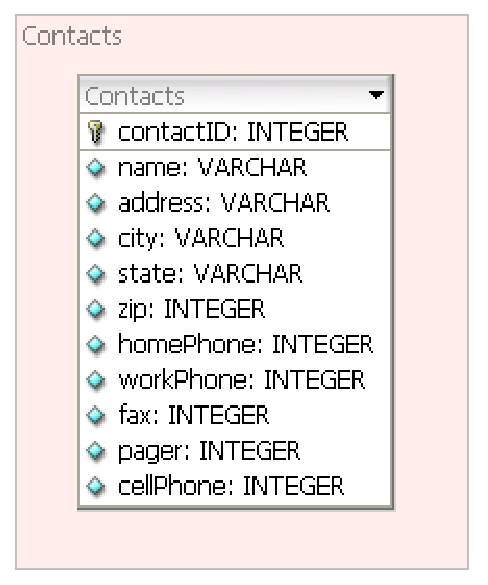
\includegraphics{Tutorials/images/BadContactModel.pdf}}
	\caption{A poorly designed contacts database}
	\label{fig:BadContactModel}
\end{figure}

\subsection{Going back and doing it right}

This program needs to store information on customers.  First, we need to define the 
customer:
\begin{quote}
A customer is any person who has done business with us or who we think might do 
business with us in the future. We need to know this person�s name, address, phone 
numbers, and email address in order to contact him or her.
\end{quote}

\subsubsection{Tackling the Name}

Ok, so we have this definition and we have the crappy model in the previous section 
that fits this definition.  At first glance putting the name in it's own field seems like 
a very good idea.  It only takes up one column so we have less data points to store 
and our SQL statements are smaller.  But what about searchability?  Let's take the 
name John Smith for example.  I, as a user can enter the name as "John Smith", 
"Smith, John", "John W. Smith", "Mr. John Smith", and "Mr. Smith, John" and they 
would all be semantically correct.  However, if I do a search and look for name being 
"John Smith", what are the chances that I am going to come back with the proper 
entry?  Slim I would say, and for database we need absolutely certainty.  The problem 
stems from us trying to lump two nibbles of information into one data field.  Suppose 
we separate the name into firstName and lastName.  Now, it doesn't matter how the 
user semantically writes names, searching for lastName="Smith" and firstName="John" 
should return the proper result each time.  The updated model is shown in Fig.
~\ref{fig:NameUpdateModel}.

\begin{figure}[ht]
	\centering
	 \scalebox{.6}{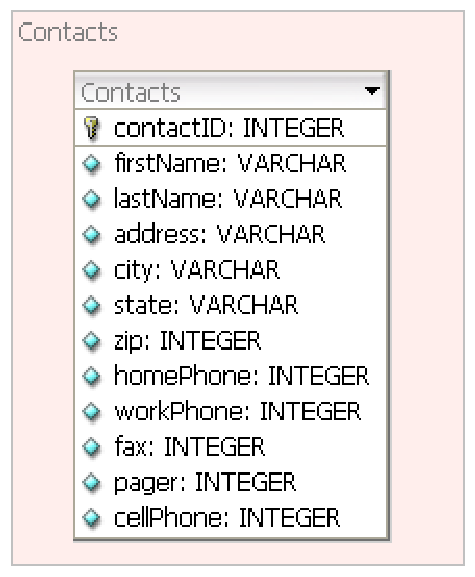
\includegraphics{Tutorials/images/NameUpdateModel.pdf}}
	\caption{Updated Name Fields}
	\label{fig:NameUpdateModel}
\end{figure}

\subsubsection{Tackling the Phone Numbers}

Next, let's look just at the phone data fields for now.  To help illustrate the problem, 
we will look at some sample rows plugged into the table.  Table 
~\ref{tbl:PhoneSampleData} shows us the data (with address info removed to 
reduce it).  Do you see anything wrong with it?  

\begin{center}
	\tablefirsthead
	{%
		\hline
		\multicolumn{1}{|c}{firstName} &
		\multicolumn{1}{|c}{lastName} &
		\multicolumn{1}{|c}{homePhone} &
		\multicolumn{1}{|c}{workPhone} &
		\multicolumn{1}{|c}{cellPhone} &
		\multicolumn{1}{|c}{fax} &
		\multicolumn{1}{c|}{pager} \\
		\hline
		\hline
	}
	
	\tablehead
	{%
		\hline
		\multicolumn{7}{|l|}{\small\sl continued from previous page}\\
		\hline
		\multicolumn{1}{|c}{firstName} &
		\multicolumn{1}{|c}{lastName} &
		\multicolumn{1}{|c}{homePhone} &
		\multicolumn{1}{|c}{workPhone} &
		\multicolumn{1}{|c}{cellPhone} &
		\multicolumn{1}{|c}{fax} &
		\multicolumn{1}{c|}{pager} \\
		\hline
		\hline
	}
	
	\tabletail
	{%
		\hline
		\multicolumn{7}{|r|}{\small\sl continued on next page}\\
		\hline
	}
	
	\tablelasttail{\hline}
	\bottomcaption{Example phone data for a bad database}
 	\label{tbl:PhoneSampleData}
	
	\begin{supertabular}{|l|l|l|l|l|l|l|}
		George & Barnes & 562-874-1234 & & 310-999-3628 & & \\ \hline
		Susan & Noble & 562-975-3388 & 714-847-3366 & & & \\ \hline
		Erwin & Star & & & & 714-997-5885 & 714-997-2428 \\ \hline
		Alice & Buck & & 562-577-1200 & 562-561-1921 & & \\ \hline
		Frank & Borders & 714-968-8201 & & & & \\ \hline
		Hanna & Diedrich & & & 562-786-7727 & & \\
	\end{supertabular}
\end{center}

There are at least two very large problems here:
\begin{itemize}
	\item There is no contact on that list that has every phone number.  The majority
		of the contacts will only have one or two numbers, which means there are a 
		lot of fields that are NULL (NULL being the constant value that means the field 
		hasn't been assigned a value).  We want to eliminate all of the unnecessary 
		NULL values in our design.
	\item Even though we provide 5 phone number fields, someone will want another 
		phone number added sooner or later.  If we want to add another phone number 
		field we actually have to change the table structure.  This is very bad design.  
		Information that colud change, like these phone numbers columns, should be kept 
		as data in a table rather than a part of the data structure.
\end{itemize}

When looking closer we realize that we don't have five single attributes.  There is 
rather a single repeated attribute, phone number.  The phone has an attribute of it's 
own telling us the type of number that it is.  This is sometimes called a weak entity, 
though it is easier to think of it as a class within a class.  So, we will pull the phone 
number out into it's own table.  I neglected to show email because it follows the same 
structure as the phone numbers.  A person can have a work email, home email, and 
more.  When the phone numbers and the emails are pulled out of the contacts table, 
we get the model shown in Fig.~\ref{fig:PhoneUpdateModel}.  As we can see, this 
already looks cleaner.

\begin{figure}[ht]
	\centering
	 \scalebox{.6}{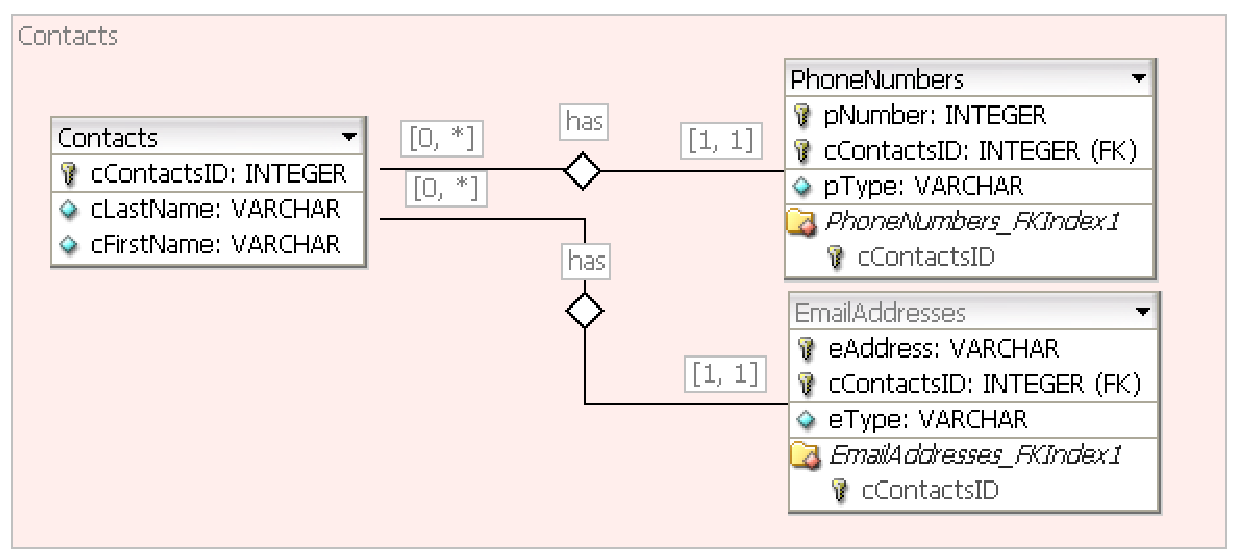
\includegraphics{Tutorials/images/PhoneUpdateModel.pdf}}
	\caption{Updated the phone fields for the contacts database}
	\label{fig:PhoneUpdateModel}
\end{figure}

\subsubsection{Tackling the Address}

Now we need to add the address fields into our database.  But should they just be 
added to the contacts table like in the previous design?  Or do they need to be 
normalized like the phone numbers and email addresses?  It's not obvious at first, but 
we need to normalize the database.  Let's look at Table~\ref{tbl:AddressSampleData} 
which shows some sample data from the contacts table with the address fields.  
Notice the repeated city and state attributes?  This is not only redundant data, but 
we also have increased potential for typos (notice the typo in row 5?).  
\begin{center}
	\tablefirsthead
	{%
		\hline
		\multicolumn{1}{|c}{firstName} &
		\multicolumn{1}{|c}{lastName} &
		\multicolumn{1}{|c}{street} &
		\multicolumn{1}{|c}{zipCode} &
		\multicolumn{1}{|c}{city} &
		\multicolumn{1}{c|}{state} \\
		\hline
		\hline
	}
	
	\tablehead
	{%
		\hline
		\multicolumn{6}{|l|}{\small\sl continued from previous page}\\
		\hline
		\multicolumn{1}{|c}{firstName} &
		\multicolumn{1}{|c}{lastName} &
		\multicolumn{1}{|c}{street} &
		\multicolumn{1}{|c}{zipCode} &
		\multicolumn{1}{|c}{city} &
		\multicolumn{1}{c|}{state} \\
		\hline
		\hline
	}
	
	\tabletail
	{%
		\hline
		\multicolumn{6}{|r|}{\small\sl continued on next page}\\
		\hline
	}
	
	\tablelasttail{\hline}
	\bottomcaption{Example phone data for a bad database}
 	\label{tbl:AddressSampleData}
	
	\begin{supertabular}{|l|l|l|l|l|l|}
		George & Barnes & 1254 Bellflower & 90840 & Long Beach & CA \\ \hline
		Susan & Noble & 1515 Palo Verde & 90840 & Long Beach & CA \\ \hline
		Erwin & Star & 17022 Brookhurst & 92708 & Fountain Valley & CA \\ \hline
		Alice & Buck & 3884 Atherton & 90836 & Long Beach & CA \\ \hline
		Frank & Borders & 10200 Slater & 92708 & Fountian Valley & CA \\ \hline
		Hanna & Diedrich & 1699 Studebaker & 90840 & Long Beach & CA \\ \hline
	\end{supertabular}
\end{center}

The problem here lies in the fact that the city and the state are functionally 
dependent on the zip code.  This means that I can uniquely determine the value of 
the city and state attributes if given a table that has data plus the value of the zip 
code.  The zip code is what is called a subkey of the Contacts table.  It is not a 
super key, but it functionally determines the city and state.  In other words, if you 
know the zip code, you can always find the city and state.  In order to solve this 
problem, we need to:
\begin{itemize}
	\item Remove all of the attributes dependent on the subkey and put them into a 
		new table called ZipLocations.
	\item Set the primary key attribute of the ZipLocations table as a duplicate of the
		subkey zipCode.
	\item Leave a copy of the zipCode attribute in the Contacts table. The zipCode 
		attribute is no longer a subkey because we moved every attribute that was 
		dependent on it into a ZipLocations table.  It now becomes a foreign key and 
		there is a many-to-one relationship between the Contacts table and the 
		ZipLocations table.
\end{itemize}

The updated database model can be seen in Fig.~\ref{fig:FinalContactModel}.

\begin{figure}[ht]
	\centering
	 \scalebox{.6}{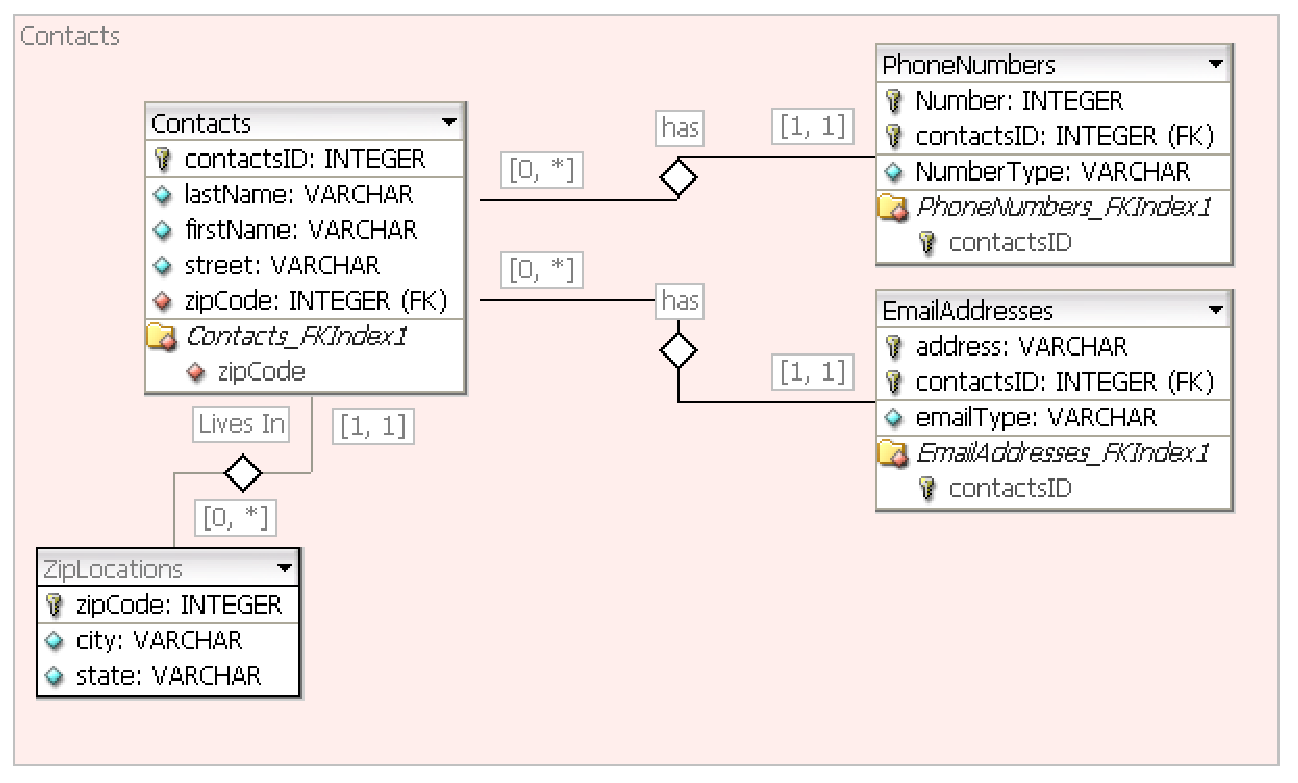
\includegraphics{Tutorials/images/FinalContactModel.pdf}}
	\caption{The Final Design For The Contacts Database}
	\label{fig:FinalContactModel}
\end{figure}

\section{Database Implementation}

Dabo supports several databases.  Dabo takes care of all of the interfacing so each 
database is can be mated plug and play with the application.  While we have several 
choices for databases we will be using a MySQL database for this program because 
it is free for non-commercial applications and available to everyone.  This book 
assumes some knowledge of setting up and administering database systems.  These 
topics will be outside the scope of this book.  There are several excellent tutorials 
out there on how to do this.

Many people think that Dabo provides framework methods to create tables and 
administer a database.  Dabo does not provide any of this functionality.  This is in 
part due to the specific nuances of SQL for different implementations and in part 
due to the abundance of database administration programs that do a spectacular 
job already.  We felt this need was more of a systems administrator job rather than 
a developer's job.  So, please set up this database and it's table before continuing 
to the next section.

\section{Backend Interfacing with Biz Objects}

By now, we hope that you have been successful setting up the MySQL database 
with the correct tables.  If not, please consult the internet for ways in which to do 
this.  We have this database, now how exactly do we interface to it?  If you remember 
from the introduction Dabo provides 3 tiers of functionality: the database layer, the 
business rules layer, and the user interface layer.  For most programs, we can 
completely ignore the database layer.

The database layer (db layer) controls all of the access to the various databases. 
It's sole functionality is to send and receive data from the database.  The good thing 
for developers that use the framework is that you can largely ignore this layer as it's
functionality is accessed through the business rules layer (biz layer).

